% Draft in a NeurIPS-like layout. For submission, replace the preamble's layout block with the venue's official
% style file (e.g. \usepackage{neurips_2026}) and remove \usepackage{geometry} and the font line.
\documentclass[10pt]{article}

% ---- layout (NeurIPS-like) ----
\usepackage[letterpaper, textwidth=5.5in, textheight=9in, top=1in, headheight=12pt, headsep=25pt, footskip=30pt]{geometry}
\usepackage{times}
% ---- packages ----
\usepackage[T1]{fontenc}
\usepackage{amsmath, amssymb}
\usepackage{graphicx}
\usepackage{booktabs}
\usepackage{xcolor}
\usepackage[numbers, sort&compress]{natbib}
\usepackage{tikz}
\usetikzlibrary{arrows.meta, positioning, fit, calc}
\usepackage[font=small, labelfont=bf]{caption}
\usepackage[hidelinks]{hyperref}

\newcommand{\pending}[1]{\textcolor{red}{[pending: #1]}}
\newcommand{\tbd}{\textcolor{red}{TBD}}
\newcommand{\csq}{count$^2$}

\title{Count-Squared Spiking Attention:\\ A Multiplier-Free Spiking Transformer for Symbolic Music Generation}
\author{Anonymous Authors}
\date{}

\begin{document}
\maketitle

\begin{abstract}
Spiking transformers promise energy-efficient sequence modelling, but two obstacles keep them from being
multiplier-free in practice: spike-count attention without a softmax cannot focus on the few keys that matter, and
the additive residual stream carries multi-bit values that turn the next layer's accumulations back into
multiplications. We propose \emph{\csq{} attention}, which weights each key by the square of its query--key spike
overlap. It sharpens attention without a cut-off, avoids the training instability we observe with learned count
thresholds, and costs one 33-entry lookup table. Combined with a fully integer datapath --- leading-bit shift coding
of the residual stream, int8 weights, an integer L1 normalisation with a 16-entry reciprocal table, and
normalisation gains folded into 12-bit leaky integrate-and-fire neurons --- every spiking block runs on shifts,
additions and one small multiply per normalised element. On the folk-rnn corpus of 23{,}600 Irish folk tunes in ABC
notation, the quantization-aware-trained model reaches 1.412 bits/token on the test split, ahead of a
folk-rnn-style LSTM (1.591) and closing 84\% of the gap between a plain spiking baseline (2.402) and its ANN teacher
(1.220); 85\% of the bars it generates have the correct length. A bit-exact integer reference model reproduces this
result exactly. An energy analysis that counts memory traffic and compares against int8 baselines, rather than
fp32 ones, puts the spiking model at roughly 7$\times$ below fp32 models but only 1.2--1.65$\times$ below an int8
transformer, and shows that the advantage depends on skipping zero inputs.
\end{abstract}

% =====================================================================================================
\section{Introduction}

Spiking neural networks (SNNs) communicate with binary spikes, so their synaptic operations can be accumulations
instead of multiply--accumulates. Spiking transformers \citep{zhou2023spikformer, yao2023spikedriven,
zhou2023spikingformer} bring this idea to attention-based models, and spiking language models
\citep{zhu2023spikegpt, wta2026} extend it to generation. Three issues stand between these models and a truly
multiplier-free implementation, and a fourth affects how their efficiency is reported.

\textbf{Attention without a softmax is diffuse.} In spiking self-attention, the score between a query and a key is
the number of spikes they share. Without a softmax there is no mechanism that concentrates attention on a few
strong matches, and our measurements show that spike-count attention stays far broader than the attention of a
same-shape ANN. A natural fix --- cutting off weak matches with a (learned) count threshold, a soft form of
winner-take-all --- turns out to be unstable: because counts are integers, a threshold that crosses an integer
flips the attention pattern of a whole head at once.

\textbf{The residual stream is not binary.} Adding spike tensors along the residual path produces small integers
(0--13 in our model), so the layers that read the residual stream perform integer-by-weight multiplications
\citep{zhou2023spikingformer, yao2023spikedriven}. In our model these layers account for 78\% of all synaptic
events.

\textbf{Normalisation needs division.} Layer normalisation in front of every spiking neuron requires a per-vector
division and a per-element gain.

\textbf{Energy comparisons are often against fp32.} Counting additions against fp32 multiply--accumulates
overstates the benefit of spikes; recent work argues for comparisons against quantized ANNs that include memory
traffic \citep{yan2024reconsidering, shen2024efficient}.

\paragraph{Contributions.}
\begin{itemize}
  \item \textbf{\csq{} spiking attention}: keys are weighted by the squared spike overlap. It improves test
        bits/token by 0.10 over a learned count threshold and raises correct bar lengths in generated tunes from
        50\% to 58\%, with stable training (Section~\ref{sec:csq}).
  \item \textbf{A multiplier-free integer datapath} for the spiking block: leading-bit shift coding of the
        residual stream, int8 weights with one scale per tensor, integer L1 normalisation with a 16-entry
        reciprocal table, and normalisation gain and bias folded into 12-bit LIF neurons. With quantization-aware
        training (QAT) it costs 0.021 bits/token against an equally trained float model, and a bit-exact integer
        reference reproduces it exactly (Section~\ref{sec:datapath}).
  \item \textbf{The first spiking transformer for symbolic music}, to our knowledge: on the folk-rnn ABC corpus
        it outperforms a folk-rnn-style LSTM in test bits/token (1.412 vs.\ 1.591), with tune-structure metrics
        close to the reference models (Section~\ref{sec:results}).
  \item \textbf{An energy analysis against int8 baselines} that includes memory traffic and a sensitivity sweep
        over memory cost: the spiking model is about 7$\times$ below fp32 models but 1.2--1.65$\times$ below int8
        ones, and only with zero-skipping (Section~\ref{sec:energy}).
\end{itemize}

% =====================================================================================================
\section{Related work}

\paragraph{Spiking transformers.} Spikformer \citep{zhou2023spikformer} introduced spiking self-attention with
binary queries, keys and values and no softmax. The Spike-driven Transformer \citep{yao2023spikedriven} replaces
the score matrix with mask-and-add operations and moves residual connections onto membrane potentials so that all
layers receive binary spikes; Spikingformer \citep{zhou2023spikingformer} pursues the same goal of avoiding the
multi-bit residual stream of SEW-style shortcuts \citep{fang2021sew}. Other work replaces or restores parts of the
softmax: bipolar attention with a Shiftmax \citep{bipolar2025}, Laplacian kernels over first-spike times
\citep{lapis2026}, and addition-only attention with full-precision keys \citep{a2os2a2025}. Winner-take-all
spiking attention for language modelling \citep{wta2026} is the closest to our threshold experiments. We are not
aware of prior work that weights spiking attention by squared overlap counts. Instead of moving the residual onto
membranes, our shift coding keeps the standard additive residual and removes the multiplications by rounding.

\paragraph{Spiking language models.} SpikeGPT \citep{zhu2023spikegpt} trains a spiking RWKV-style model for text
generation; we trained a spiking transformer on enwik8 in an earlier phase of this work and found it behind
SpikeGPT (1.447 vs.\ about 1.26 bits/character), which motivated the architectural changes studied here.

\paragraph{Symbolic music generation.} folk-rnn \citep{sturm2016folkrnn} trained LSTMs on ABC transcriptions of
Irish folk tunes; transformers now dominate ABC modelling \citep{qu2024mupt, wang2025notagen}. Spiking models of
music exist but work on pitch sequences rather than ABC text, as far as we know.

\paragraph{Efficiency evaluation and quantization.} \citet{yan2024reconsidering} and \citet{shen2024efficient}
show that SNN energy claims must be made against quantized ANNs and include memory access; our analysis follows
that advice. Our datapath builds on integer-only quantization \citep{jacob2018quantization}, shift-based
multiplication \citep{elhoushi2021deepshift} and straight-through gradients \citep{bengio2013estimating}.

% =====================================================================================================
\section{Model}
\label{sec:model}

\begin{figure}[t]
\centering
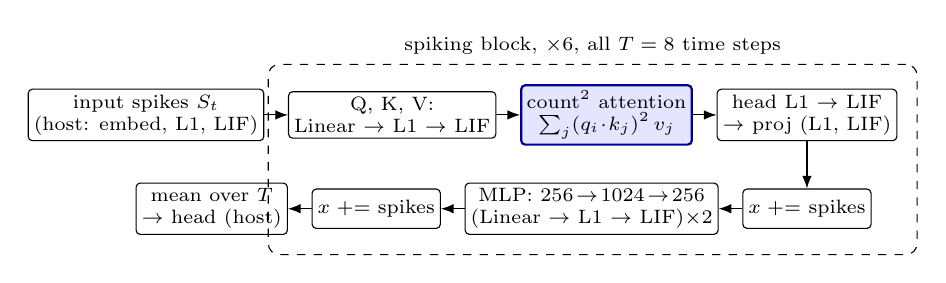
\begin{tikzpicture}[font=\scriptsize, node distance=2.2mm and 3mm,
    box/.style={draw, rounded corners=1.5pt, minimum height=5mm, inner sep=2pt, align=center},
    acc/.style={box, fill=blue!10, draw=blue!60!black, thick},
    arr/.style={-{Latex[length=1.6mm]}, thin}]
  \node[box] (in) {input spikes $S_t$\\(host: embed, L1, LIF)};
  \node[box, right=of in] (qkv) {Q, K, V:\\Linear $\to$ L1 $\to$ LIF};
  \node[acc, right=of qkv] (att) {\csq{} attention\\$\sum_j (q_i\!\cdot\!k_j)^2\, v_j$};
  \node[box, right=of att] (hn) {head L1 $\to$ LIF\\$\to$ proj (L1, LIF)};
  \node[box, below=6mm of hn] (add1) {$x \mathrel{+}= $ spikes};
  \node[box, left=of add1] (mlp) {MLP: $256\!\to\!1024\!\to\!256$\\(Linear $\to$ L1 $\to$ LIF)$\times$2};
  \node[box, left=of mlp] (add2) {$x \mathrel{+}= $ spikes};
  \node[box, left=of add2] (out) {mean over $T$\\$\to$ head (host)};
  \draw[arr] (in) -- (qkv); \draw[arr] (qkv) -- (att); \draw[arr] (att) -- (hn);
  \draw[arr] (hn) -- (add1); \draw[arr] (add1) -- (mlp); \draw[arr] (mlp) -- (add2); \draw[arr] (add2) -- (out);
  \node[draw, dashed, rounded corners, fit=(qkv)(att)(hn)(add1)(mlp)(add2), inner sep=2.5mm,
        label={[font=\scriptsize]above:spiking block, $\times 6$, all $T=8$ time steps}] {};
\end{tikzpicture}
\caption{Model overview. Every arrow inside a block carries binary spikes, except the residual stream $x$, which
holds counts 0--13. Q/K/V and the first MLP layer read the residual stream; the projection and second MLP layer
read spikes.}
\label{fig:arch}
\end{figure}

\paragraph{Spiking block.} Our model follows the pre-normalised transformer layout with spiking components
(Figure~\ref{fig:arch}). A token is simulated for $T$ time steps. Every linear layer is followed by an L1 layer
normalisation (mean subtraction and division by the mean absolute deviation, MAD) and a leaky integrate-and-fire
(LIF) neuron with time constant 2, threshold 1 and soft reset:
\begin{equation}
  v_t = \tfrac{1}{2}(v_{t-1} + x_t), \qquad s_t = [v_t \ge 1], \qquad v_t \leftarrow v_t - s_t .
  \label{eq:lif}
\end{equation}
Gradients pass the spike function through a sigmoid surrogate \citep{neftci2019surrogate}. Attention operates
per time step on binary queries $q_i$, keys $k_j$ and values $v_j$ of 8 heads with 32 channels each; the read-out
averages the residual stream over the $T$ steps and applies a linear head. The model has 6 blocks of width 256
and MLP width 1{,}024 (4.89M parameters) and a context of 256 tokens.

\subsection{\csq{} attention}
\label{sec:csq}

In spiking self-attention \citep{zhou2023spikformer} the score $c_{ij} = q_i \cdot k_j$ counts the channels in
which query $i$ and key $j$ both spiked, and the output is $\sum_{j \le i} c_{ij} v_j$. We use instead
\begin{equation}
  a_i = \sum_{j \le i} c_{ij}^{\,2}\, v_j , \qquad c_{ij} = \mathrm{popcount}(q_i \wedge k_j) \in \{0, \dots, 32\},
\end{equation}
followed by a per-head L1 normalisation and an LIF neuron. Squaring lets strong matches dominate (a 4-channel match
counts 16 times a 1-channel match instead of 4 times) while weak matches still contribute. In hardware the square
of a 6-bit count is a 33-entry table, and pairs with $c_{ij}=0$ (75\% of pairs in our model) are skipped.

\paragraph{Why not a threshold?} The obvious alternative is to discard weak matches: keep $c_{ij}$ only if
$c_{ij} \ge \theta_h$, with a learned per-head $\theta_h$ and a sigmoid surrogate gradient. Two properties of
integer counts make this fragile. First, all $\theta \in (1, 2]$ produce the same forward pass (they drop exactly
the 1-channel matches), so gradient descent drifts $\theta$ inside this band without effect
(Figure~\ref{fig:theta}). Second, when $\theta$ reaches an integer the forward pass changes abruptly: in a model
with thresholds on all heads, three heads of block 4 settled at exactly $\theta = 2.00$, where moving $\theta$ by
0.01 changed the model's output distribution by a KL divergence of 7.6 nats and quadrupled the block's gradient
norm. Training showed gradient spikes of 8--14$\times$ the running average in that block. Fixing $\theta$ removes
the instability but makes the cut too strict (Table~\ref{tab:attn}). \csq{} attention keeps the sharpening and
has no discontinuity.

\begin{figure}[t]
\centering
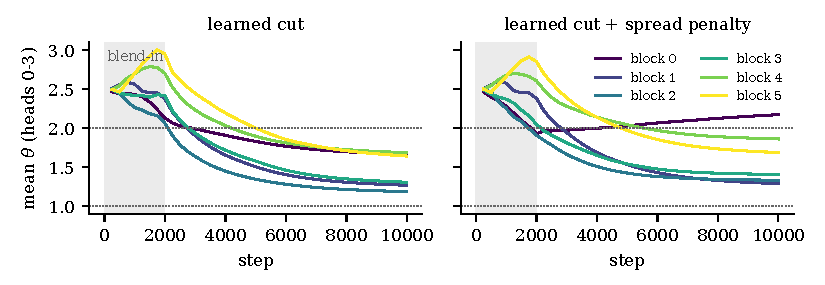
\includegraphics[width=\linewidth]{figures/theta.pdf}
\caption{Learned count thresholds drift down toward 1 after the blend-in (shaded) unless a spread penalty rewards
cutting; dotted lines mark the integer boundaries where the forward pass changes.}
\label{fig:theta}
\end{figure}

\subsection{Training}
\label{sec:training}

\paragraph{Distillation.} An ANN of the same shape \citep{vaswani2017attention} serves as teacher
\citep{hinton2015distilling}. The loss mixes cross-entropy with the KL divergence to the teacher's output
distribution and a \emph{reverse} KL between the student's normalised attention rows and the teacher's softmax
attention on 64 sampled query rows \citep{jiao2020tinybert, wang2020minilm}. The reverse (mode-seeking) direction
mattered: the forward direction flattened spike-count attention.

\paragraph{Spread penalty.} We add the normalised entropy of attention rows, $H(\hat{a}_i)/\log(i+1)$, as a
penalty with weight 0.1. It pushes attention toward the teacher's sharpness and gives a threshold a reason to rise
(Figure~\ref{fig:theta}).

\paragraph{Homeostasis and dropout.} Units that fire in fewer than 1\% or more than 50\% of steps have their
normalisation bias nudged toward the range \citep{turrigiano2004homeostatic}, with a capped cumulative shift; this
removed nearly all never-firing units. Spike dropout \citep{srivastava2014dropout} on each block's attention and
MLP outputs (inverted, training only) was the single most effective regulariser in long runs.

\paragraph{Schedules.} After a 2{,}000-step ramp-in of \csq{} and the penalty, the output-KL weight, attention-KL
weight and spread penalty decay linearly to zero at step 30{,}000 while the surrogate sharpness rises from 2 to 4;
training continues on cross-entropy to step 50{,}000. Abrupt schedule changes broke training (Appendix~\ref{app:hp}).

\subsection{Multiplier-free integer datapath}
\label{sec:datapath}

\paragraph{Shift-coded residual inputs.} The residual stream holds counts $r \in \{0, \dots, 13\}$. We replace
each by its leading bit, rounded on the first dropped bit and saturated at 8, so $r \mapsto \{0,1,2,4,4,4,8,\dots\}$
and every product $w \cdot r$ becomes a shift of the int8 weight by 0--3 places. Values that would round to 16 occur
for 0.001\% of inputs, so the saturation is free.

\paragraph{Integer normalisation.} With one int8 scale per weight tensor, the normalisation removes the scale, so
it operates directly on integer accumulators. Mean and MAD are integer sums followed by a shift (all widths are
powers of two) and rounding; the MAD is held in 12 bits. Its reciprocal comes from a leading-one detector and a
16-entry table indexed by the four bits after the leading one, so the only multiplier in the block is the
19$\times$6-bit product of the centred value and the table entry, rounded to a 12-bit Q4.7 output.

\paragraph{Folded LIF.} Because Equation~\ref{eq:lif} is linear below threshold, the normalisation gain $\gamma$
and bias $\beta$ fold into each neuron: in units of $\gamma$ the state evolves as
$u \leftarrow (u + n + \beta/\gamma) \gg 1$, fires when $\gamma(u - 1/\gamma) \ge 0$ and subtracts $1/\gamma$ on a
spike, all in Q4.7. This is exact in real arithmetic. The 40 neurons (0.26\%) with $|\gamma| < 0.05$ would need
thresholds beyond the 12-bit range; their input is negligible and setting them to never fire costs nothing.

\paragraph{Quantization-aware training and reference model.} We fine-tune with the whole datapath in the forward
pass and straight-through gradients \citep{bengio2013estimating}. A NumPy integer model with explicit rounding
(half up) and saturation reproduces the PyTorch datapath on 100\% of block outputs and gives an identical test
score; it doubles as the specification and test-vector generator for hardware.

% =====================================================================================================
\section{Experimental setup}
\label{sec:setup}

\paragraph{Data.} The folk-rnn corpus \citep{sturm2016folkrnn}: about 23{,}600 tunes transposed to C, tokenised
into 135 ABC symbols (one token per note, duration, bar line, repeat sign, meter or mode) plus end-of-tune, split
90/5/5 by tune.

\paragraph{Metrics.} Test bits per token over the full test split with a 256-token sliding window (stride 128).
For generation, 500 tunes sampled at temperature 1 are checked automatically: the share of bars whose durations
match the meter (first and last bars excluded), a single valid meter and mode header, balanced repeat signs, and a
final tonic.

\paragraph{Baselines.} The ANN teacher (same shape, 4.87M parameters, 10k steps) and a folk-rnn-style LSTM
\citep{hochreiter1997lstm} with 3 layers of 512 units and one-hot input (5.60M parameters, 30k steps). For int8
comparisons both are quantized after training: the ANN with int8 weights and activations at every linear input
and on Q/K/V, the LSTM with int8 weights and hidden state.

\paragraph{Training.} AdamW, learning rate $7\times10^{-4}$ with cosine decay, batch $64 \times 256$ tokens, bf16;
the final model trains 50k steps at $T=8$ and is then fine-tuned for 5k steps with QAT (Appendix~\ref{app:hp}).
\pending{all results below are single runs; seed repeats are listed in Table~\ref{tab:seeds}.}

% =====================================================================================================
\section{Results}
\label{sec:results}

\begin{table}[t]
\centering
\caption{Main results on the folk-rnn test split. Tune columns from 500 generated tunes (about $\pm$2--3 points
sampling noise). Float spiking = the final model fine-tuned 5k steps in float; PTQ = the same model quantized after
training; QAT = fine-tuned with the integer datapath.}
\label{tab:main}
\small
\begin{tabular}{lcccccc}
\toprule
Model & Params & Bits/token $\downarrow$ & Correct bars & Header & Repeats & Ends on C \\
\midrule
Real test tunes & --- & --- & 89.9 & 100 & 80.3 & 62.8 \\
\midrule
ANN teacher, fp32 & 4.87M & \textbf{1.220} & 88.9 & 98.8 & 78.2 & 55.8 \\
ANN teacher, int8 & 4.87M & 1.225 & \tbd & \tbd & \tbd & \tbd \\
LSTM 3$\times$512, fp32 & 5.60M & 1.591 & \textbf{90.9} & 100 & 78.4 & 57.8 \\
LSTM 3$\times$512, int8 & 5.60M & 1.596 & \tbd & \tbd & \tbd & \tbd \\
\midrule
Spiking baseline (plain counts, 10k) & 4.89M & 2.402 & 35.4 & 98.4 & 69.8 & 46.8 \\
Spiking, float & 4.89M & 1.392 & \tbd & \tbd & \tbd & \tbd \\
Spiking, PTQ (integer) & 4.89M & 1.433 & \tbd & \tbd & \tbd & \tbd \\
Spiking, QAT (integer) & 4.89M & 1.412 & 85.1 & 99.2 & 72.0 & \textbf{59.2} \\
\bottomrule
\end{tabular}
\end{table}

\paragraph{Main results.} The integer spiking model reaches 1.412 bits/token (Table~\ref{tab:main}), 0.18 better
than the LSTM and 0.19 behind the ANN teacher, closing 84\% of the gap between the plain spiking baseline and the
teacher. Its tunes are structurally sound: 99\% have a valid header and 85\% of bars have the correct length,
against 89--91\% for the ANN and LSTM. Ranking by bits/token does not predict tune structure: the LSTM has the worst
score among the reference models but the best bars, headers and repeats.

\begin{figure}[t]
\centering
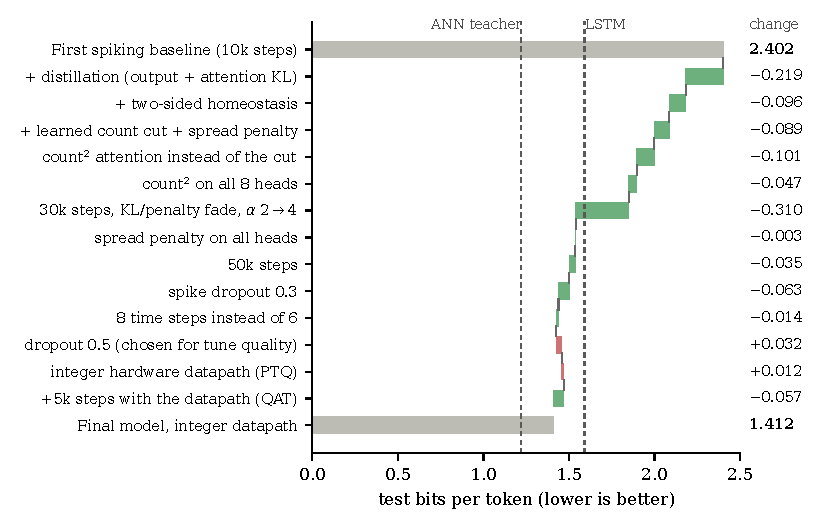
\includegraphics[width=0.92\linewidth]{figures/progression.pdf}
\caption{Test bits/token along the main line of development, one change at a time (single runs; 10k steps until
the 30k row).}
\label{fig:progression}
\end{figure}

\paragraph{Development path.} Figure~\ref{fig:progression} decomposes the improvement. Training length with
decaying distillation and penalty terms gave the largest single step ($-0.31$), followed by distillation
($-0.22$) and \csq{} attention ($-0.10$ over a learned cut with the spread penalty). Spike dropout removed late
overfitting: at 50k steps the train/validation gap fell from 0.35 to 0.12 bits/token. A stronger, longer-trained
teacher (1.199 vs.\ 1.220) did not help the student (+0.012), suggesting the student, not the teacher, is the
bottleneck. These are sequential additions under different budgets; a one-at-a-time ablation of the final recipe
is in Table~\ref{tab:ablation}.

\begin{table}[t]
\centering
\caption{Attention variants with distillation and homeostasis, $T=6$, 10k steps, single runs. The spread penalty
(weight 0.1) and the cut or square apply to heads 0--3 unless marked ``8 heads''.}
\label{tab:attn}
\small
\begin{tabular}{lccl}
\toprule
Attention & Bits/token $\downarrow$ & Correct bars & Note \\
\midrule
Plain spike counts & 2.087 & 51.6 & \\
Learned cut & 2.075 & 45.9 & $\theta$ drifts to the (1,2] band \\
Spread penalty only & 2.064 & 50.3 & \\
Fixed cut $\theta=2.5$ + spread, 8 heads & 2.038 & 43.2 & stable, too strict \\
Learned cut + spread, 8 heads & 2.005 & 48.9 & gradient spikes 8--14$\times$ \\
Learned cut + spread & 1.998 & 49.6 & \\
\csq{} + spread & 1.897 & \textbf{57.5} & \\
\csq{}, 8 heads + spread & \textbf{1.850} & 54.8 & \\
\bottomrule
\end{tabular}
\end{table}

\paragraph{Attention variants.} Table~\ref{tab:attn} isolates the attention mechanism. The spread penalty helps
only with a mechanism to act through: alone it gains 0.023, with a learned cut 0.089, and \csq{} adds another
0.101. \csq{} is also the only variant that raises bar correctness above the 50\% plateau of the 10k-step models.
Raising the penalty from 0.1 to 0.3 changed nothing (1.847), as \csq{} already provides the sharpening.

\begin{table}[t]
\centering
\caption{Seed repeats of the attention comparison (10k steps, $T=6$): mean $\pm$ standard deviation over 3 seeds.}
\label{tab:seeds}
\small
\begin{tabular}{lcc}
\toprule
Attention & Bits/token & Correct bars \\
\midrule
Plain spike counts + spread & \tbd & \tbd \\
Learned cut + spread & \tbd & \tbd \\
\csq{} + spread & \tbd & \tbd \\
\bottomrule
\end{tabular}
\end{table}

\begin{table}[t]
\centering
\caption{One-at-a-time ablation of the final recipe (30k steps, $T=8$).}
\label{tab:ablation}
\small
\begin{tabular}{lcc}
\toprule
Variant & Bits/token & $\Delta$ \\
\midrule
Full recipe & \tbd & --- \\
$-$ \csq{} (plain counts) & \tbd & \tbd \\
$-$ spread penalty & \tbd & \tbd \\
$-$ distillation & \tbd & \tbd \\
$-$ homeostasis & \tbd & \tbd \\
$-$ spike dropout & \tbd & \tbd \\
$T=6$ instead of 8 & \tbd & \tbd \\
\bottomrule
\end{tabular}
\end{table}

\paragraph{Generalisation beyond music.} \pending{\csq{} vs.\ plain counts on enwik8 with a smaller model, 2 seeds
each; and comparisons with Spike-driven attention \citep{yao2023spikedriven} and membrane-shortcut residuals
\citep{zhou2023spikingformer} under the same recipe.}

\subsection{From float to integer}
\label{sec:quant}

\begin{table}[t]
\centering
\caption{Cost of each simplification of the datapath, applied cumulatively to the float model before QAT
(1.457 bits/token, $T=8$).}
\label{tab:quant}
\small
\begin{tabular}{lcl}
\toprule
Step & Bits/token & Hardware effect \\
\midrule
Float model & 1.457 & --- \\
+ shift-coded residual inputs & 1.464 & no multipliers in linear layers \\
+ int8 weights, one scale per tensor & 1.470 & scale never applied \\
+ integer norm, 16-entry table, Q4.7, folded LIF & 1.469 & one 19$\times$6-bit multiply per element \\
\midrule
Float fine-tune, 5k steps (control) & 1.392 & --- \\
\quad same, quantized after training (PTQ) & 1.433 & \\
QAT fine-tune, 5k steps & \textbf{1.412} & \\
\bottomrule
\end{tabular}
\end{table}

Table~\ref{tab:quant} shows that each simplification is nearly free on the float model (+0.012 in total). A 5k-step
fine-tune helps either way, so we compare QAT against a float fine-tune of the same length: QAT recovers half of the
post-training quantization loss (1.412 vs.\ 1.433), leaving 0.021 bits/token (1.5\%) as the cost of the integer
datapath. Coarser variants were not free: replacing the reciprocal table and multiply by a single power-of-two shift
cost 0.32 bits/token (0.20 from the Q/K/V normalisations alone, whose scale decides which neurons fire), a
two-term shift-add 0.016, and a 4-entry table 0.018. Rounding half up instead of half to even cost 0.0004, and
register saturation never triggered on the test split.

\subsection{Energy}
\label{sec:energy}

\begin{figure}[t]
\centering
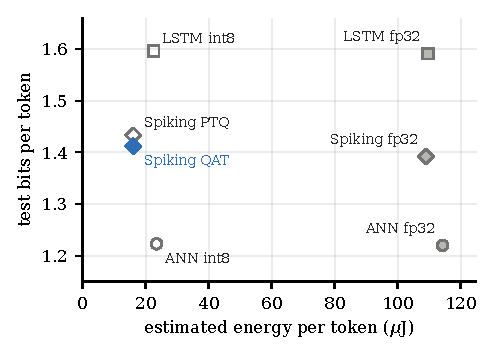
\includegraphics[width=0.6\linewidth]{figures/energy.pdf}
\caption{Test bits/token against estimated energy per generated token (256-token context, weights in on-chip
SRAM at 4 pJ/byte). Filled markers: fp32; hollow: int8; blue: the QAT spiking model.}
\label{fig:energy}
\end{figure}

\begin{table}[t]
\centering
\caption{Arithmetic energy inside the blocks per token ($\mu$J, 45 nm per-operation energies
\citep{horowitz2014energy}), with and without skipping zero inputs, and total energy including weight and cache
reads. The last column is the int8 ANN's total relative to the integer spiking model for memory costs from 1.25 to
160 pJ/byte.}
\label{tab:energy}
\small
\begin{tabular}{lccccc}
\toprule
Model & Operations/token & No skip & Skip & Total & \\
\midrule
ANN fp32 & 5.5M fp32 MACs & 25.9 & --- & 114 & \\
ANN int8 & 5.5M int8 MACs & 1.80 & --- & 23.5 & \\
LSTM int8 & 5.3M int8 MACs & 1.38 & --- & 22.6 & \\
Spiking fp32 & 11.9M MACs + 3.3M adds & 112 & 59.8 & 109 & \\
Spiking integer & 11.8M shift-adds + 3.3M adds & 2.24 & \textbf{0.95} & \textbf{16.1} & \\
\midrule
\multicolumn{5}{l}{int8 ANN total / integer spiking total, over memory costs} & 1.20--1.65$\times$ \\
\bottomrule
\end{tabular}
\end{table}

We estimate energy from measured operation counts and per-operation energies \citep{horowitz2014energy}
(Figure~\ref{fig:energy}, Table~\ref{tab:energy}; constants in Appendix~\ref{app:energy}). Three findings stand
out. First, against fp32 models the integer spiking model is about 7$\times$ cheaper across all memory costs we
tried (6.6--7.7$\times$), but against int8 baselines the margin is 1.2--1.65$\times$, in line with
\citet{yan2024reconsidering}. Second, the spiking model performs 2.7$\times$ more operations than the ANN because
every token runs for 8 time steps; in fp32 this cancels any benefit (109 vs.\ 114 $\mu$J). Third, its arithmetic is
only cheaper than an int8 ANN's when zero inputs are skipped: spike inputs are 19\% non-zero and residual inputs
58\%, so skipping cuts block arithmetic from 2.24 to 0.95 $\mu$J. The savings in total energy come mostly from
memory: each weight column is fetched once for all 8 steps and only if its input ever fires (2.78M weight reads per
token vs.\ 4.77M for the ANN), and the attention cache holds spikes.

% =====================================================================================================
\section{Analysis}
\label{sec:analysis}

\paragraph{Where the gap to the teacher lies.} Splitting test loss by token type, about 80\% of the remaining gap
to the ANN teacher is in note tokens (69\% of tokens; 1.565 vs.\ 1.343 bits) and 13\% in durations; bar lines,
repeat signs and headers are within 0.01--0.15 bits of the teacher. The spiking model has learned the structure of
the notation; it is weaker at melody.

\paragraph{Time steps.} The QAT model, trained at $T=8$, scores 1.438 at $T=6$ and 1.528 at $T=4$, giving a direct
accuracy--energy trade-off at inference time. Training at $T=8$ instead of 6 improved the float model by 0.014.

\paragraph{Generated tunes.} 72\% of generated tunes have repeat signs that pair one-to-one (80\% of real tunes).
Most failures in both are a closing repeat without an opening one, a notation habit that players read as a normal
repeat; genuinely unclosed repeats occur in 8.8\% of generated tunes against 3.2\% of real ones. 2.8\% of generated
tunes contain an ABC syntax error.

\paragraph{Activity.} The integer model fires about 20{,}200 spikes per token, with 8--30\% of neurons active per
time step depending on population and block.

% =====================================================================================================
\section{Limitations}

All reported runs are single seeds, and the main method is evaluated on one dataset \pending{see
Tables~\ref{tab:seeds} and \ref{tab:ablation} and the enwik8 experiment}. The development path in
Figure~\ref{fig:progression} adds components under different training budgets, so it does not isolate their
contributions. Energy figures are analytical estimates at 45 nm; leakage, control and data movement between units
are not modelled, and the comparison with int8 baselines is sensitive to memory cost. The model's context is 256
tokens; about 10\% of real tunes are longer and would be truncated by the hardware design, which caches keys and
values and does not slide its window. Tune quality is measured by automatic checks, not by listeners.

\section{Conclusion}

Squaring spike-overlap counts gives spiking attention the selectivity that a softmax provides in ANNs, without the
instability of learned integer thresholds. Together with shift-coded residual inputs, integer normalisation and
folded LIF neurons, it yields a spiking transformer whose blocks run on shifts and additions, outperform an LSTM on
symbolic music, and lose 0.021 bits/token to an equally trained float model. Measured honestly against int8
baselines, its energy advantage is real but modest and depends on sparse activity --- which points to sparser
residual streams as the most valuable next step.

\bibliographystyle{plainnat}
\bibliography{refs}

% =====================================================================================================
\appendix
\section{Hyperparameters}
\label{app:hp}

\begin{table}[h]
\centering
\small
\begin{tabular}{ll}
\toprule
Architecture & 6 blocks, width 256, 8 heads $\times$ 32, MLP 1{,}024, context 256, $T=8$ \\
Neurons & LIF, time constant 2, threshold 1, soft reset; sigmoid surrogate, sharpness 2 $\to$ 4 (steps 2k--30k) \\
Optimiser & AdamW, lr $7\times10^{-4}$, 500 warm-up steps, cosine to $7\times10^{-5}$ at 50k; weight decay 0.1 \\
Batch & 64 sequences $\times$ 256 tokens, bf16 \\
Gradient clipping & per block, at 3$\times$ its running average norm \\
Distillation & CE weight 0.5 $\to$ 1 and attention KL 0.15 $\to$ 0 (steps 2k--30k); 64 rows, blocks 1--5 \\
Spread penalty & 0.1 on all heads, ramped in over 2k steps, to 0 at 30k \\
Homeostasis & targets 1\%--50\% firing, rate $2\times10^{-3}$, cumulative shift cap 8 \\
Spike dropout & 0.5 (0.3 gives 0.032 lower bits/token, slightly worse tunes) \\
QAT & 5k steps, lr $10^{-4} \to 10^{-5}$, no dropout, no distillation \\
Teacher & same shape ANN, 10k steps, lr $10^{-3}$, dropout 0.2 \\
\bottomrule
\end{tabular}
\end{table}

Changing the surrogate sharpness abruptly (2 $\to$ 1 in one step) raised validation loss from 1.87 to 2.70 bits,
because Adam's second-moment estimates no longer matched the gradient scale; all schedules are therefore linear.
Introducing a hard count threshold by blending it in over 2k steps caused a jump in attention KL at the end of the
blend: the per-head normalisation rescaled the attenuated sub-threshold counts, so the cut only took effect in the
last few percent of the ramp.

\section{Energy model}
\label{app:energy}

Operation counts are measured on validation text. Per-operation energies follow \citet{horowitz2014energy}: fp32
multiply 3.7 pJ and add 0.9 pJ; int8 multiply--accumulate 0.23 pJ; an 18-bit add 0.05 pJ and a 4-way shift
multiplexer 0.01 pJ (interpolated or estimated); accumulator-buffer accesses 0.1 pJ (integer) and 0.2 pJ (fp32);
weight and cache memory 4 pJ/byte (between 32 KB and 1 MB SRAM in \citep{horowitz2014energy}). The sensitivity
sweep uses 1.25, 4, 12.5 and 160 pJ/byte. The spiking model fetches a weight column once per token for all time
steps when any of its inputs is non-zero; the ANN reads all weights once per token and a 256-entry K/V cache.

\end{document}
